\documentclass[ignorenonframetext,]{beamer}
\setbeamertemplate{caption}[numbered]
\setbeamertemplate{caption label separator}{: }
\setbeamercolor{caption name}{fg=normal text.fg}
\beamertemplatenavigationsymbolsempty
\usepackage{lmodern}
\usepackage{amssymb,amsmath}
\usepackage{ifxetex,ifluatex}
\usepackage{fixltx2e} % provides \textsubscript
\ifnum 0\ifxetex 1\fi\ifluatex 1\fi=0 % if pdftex
  \usepackage[T1]{fontenc}
  \usepackage[utf8]{inputenc}
\else % if luatex or xelatex
  \ifxetex
    \usepackage{mathspec}
  \else
    \usepackage{fontspec}
  \fi
  \defaultfontfeatures{Ligatures=TeX,Scale=MatchLowercase}
\fi
\usecolortheme{seahorse}
% use upquote if available, for straight quotes in verbatim environments
\IfFileExists{upquote.sty}{\usepackage{upquote}}{}
% use microtype if available
\IfFileExists{microtype.sty}{%
\usepackage{microtype}
\UseMicrotypeSet[protrusion]{basicmath} % disable protrusion for tt fonts
}{}
\newif\ifbibliography
\hypersetup{
            pdftitle={Association of Short-term Exposure to Air Pollution With Mortality in Older Adults},
            pdfauthor={First author Qian Di; Corresponding author Joeal D. Schwartz; Fuyu Guo Presenting},
            pdfborder={0 0 0},
            breaklinks=true}
\urlstyle{same}  % don't use monospace font for urls
\usepackage{graphicx,grffile}
\makeatletter
\def\maxwidth{\ifdim\Gin@nat@width>\linewidth\linewidth\else\Gin@nat@width\fi}
\def\maxheight{\ifdim\Gin@nat@height>\textheight0.8\textheight\else\Gin@nat@height\fi}
\makeatother
% Scale images if necessary, so that they will not overflow the page
% margins by default, and it is still possible to overwrite the defaults
% using explicit options in \includegraphics[width, height, ...]{}
\setkeys{Gin}{width=\maxwidth,height=\maxheight,keepaspectratio}

% Prevent slide breaks in the middle of a paragraph:
\widowpenalties 1 10000
\raggedbottom

\AtBeginPart{
  \let\insertpartnumber\relax
  \let\partname\relax
  \frame{\partpage}
}
\AtBeginSection{
  \ifbibliography
  \else
    \let\insertsectionnumber\relax
    \let\sectionname\relax
    \frame{\sectionpage}
  \fi
}
\AtBeginSubsection{
  \let\insertsubsectionnumber\relax
  \let\subsectionname\relax
  \frame{\subsectionpage}
}

\setlength{\parindent}{0pt}
\setlength{\parskip}{6pt plus 2pt minus 1pt}
\setlength{\emergencystretch}{3em}  % prevent overfull lines
\providecommand{\tightlist}{%
  \setlength{\itemsep}{0pt}\setlength{\parskip}{0pt}}
\setcounter{secnumdepth}{0}

\title{Association of Short-term Exposure to Air Pollution With Mortality in
Older Adults}
\author{First author Qian Di; Corresponding author Joeal D. Schwartz; Fuyu Guo
Presenting}
\date{November 29, 2020}

\begin{document}
\frame{\titlepage}

\begin{frame}{Background}

\begin{itemize}
\tightlist
\item
  US National Ambient Air Quality Standards (NAAQS) for fine particulate
  matter (PM\(_{2.5}\)) and ozone every are reviewed every 5 years.
\item
  2012 annual and 24-hour NAQQS for PM\(_{2.5}\) is 35
  \(\mu\)g/m\(^{3}\) and 12 \(\mu\)g/m\(^{3}\).
\item
  2012 8-hour NAQQS for ozone is 70 ppb, no annual stanard
\item
  Studies in large metropolitan areas have provided evidence for
  short-term exposure to PM\(_{2.5}\) and ozone were associated with
  mortality.
\end{itemize}

\end{frame}

\begin{frame}{Aim and Objectives}

\begin{itemize}
\tightlist
\item
  Aim to study the effect of short-term exposure below daily NAQQS, and
  in rural and unmonitored areas.
\item
  Aim to study the effect on sensitive subgoups such as those with low
  socio-economic status.
\end{itemize}

\end{frame}

\begin{frame}{Data source and participants}

\begin{itemize}
\tightlist
\item
  Participants: all deaths among all Medicare benficiaries from 2000 to
  2012.
\item
  Outcome: all-cause mortality. Indivdiuals with validated date of death
  between January 1, 2020 and December 31, 2012 were included.
\item
  Exposure: daily 24-hour PM\(_{2.5}\), 8-hour maximumozone, and daily
  air and dew point temperatures. Monitored data from the EPA,
  satellite-based measurements, and other data sets. Neural networks
  were used to predict 24-hour PM2.5 and 8-hour maximum ozone
  concentrations.
\item
  Warm season: April 1 to September 30, which is the specific time
  window to examine the association between ozone and mortality
\end{itemize}

\end{frame}

\begin{frame}{Case-cross over design}

\begin{itemize}
\tightlist
\item
  Usage: the design has been widely used to study the association
  between c short-term air pollution exposure and the risk of an acute
  adverse health event.
\item
  Main idea: for each individual case, exposure just before the event is
  compared with exposure at other control (``referent'') times.
\item
  Statistical method: Conditional logistic regression.
\end{itemize}

In this study\\
- Case day: date of the death. - Control days: on the same day of the
week as the case day to control for potential confounding effect by day
of week; before and after the case day to control for time trend; only
in the same month as the case day to control for seasonal and
subseasonal. - Time window: the death day and the day before death.

\end{frame}

\begin{frame}{Statistical analysis}

\begin{itemize}
\tightlist
\item
  Regression model included both pollutants as main effects and natural
  splines of air and dew point temperatures with 3 df to control for
  residual confounding by weather.
\item
  Relative risk increase (RRI) was defined as RR − 1.
\item
  The absolute risk difference (ARD) of all-cause mortality associated
  with air pollution was defined as \(\alpha \times (RR - 1)/RR\), where
  \(\alpha\) denotes the baseline daily mortality rate.
\end{itemize}

\end{frame}

\begin{frame}{Baseline characteristics}

\begin{figure}
\centering
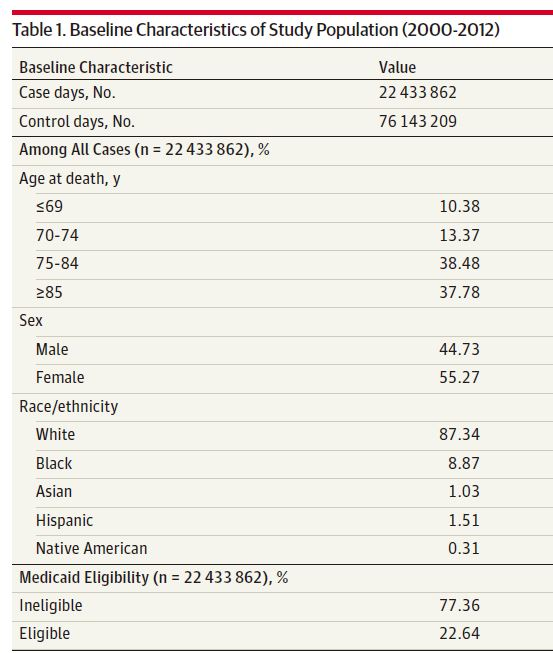
\includegraphics{p1.JPG}
\caption{Baseline Characteristics of Study Population (2000-2012)}
\end{figure}

\end{frame}

\begin{frame}{PM\(_{2.5}\) times series}

\begin{figure}
\centering
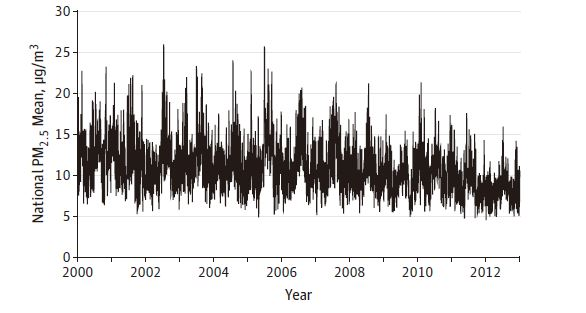
\includegraphics{p2.JPG}
\caption{Daily mean fine particulate matter PM\(_{2.5}\) concentrations}
\end{figure}

\end{frame}

\begin{frame}{Ozone time series}

\begin{figure}
\centering
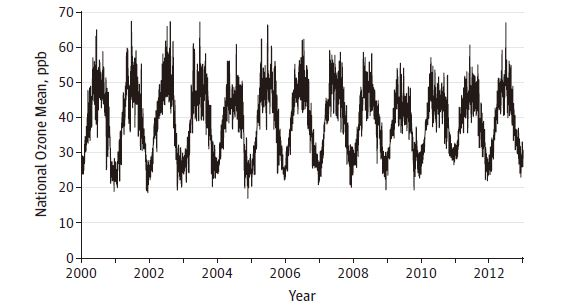
\includegraphics{p3.JPG}
\caption{Daily mean 8-hour maximum ozone concentrations}
\end{figure}

\end{frame}

\begin{frame}{Regression result}

\begin{figure}
\centering
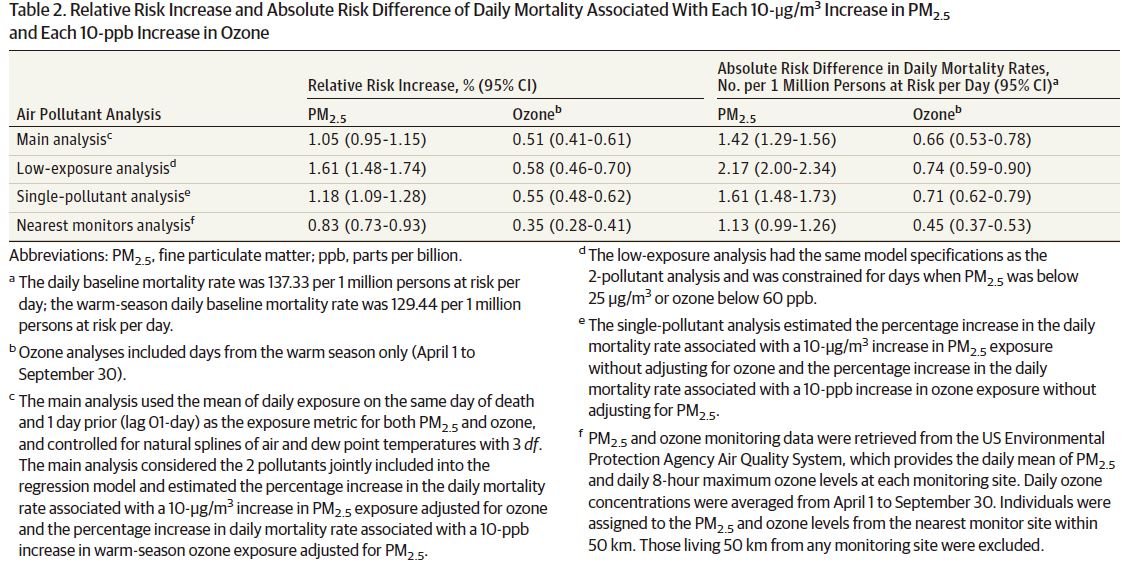
\includegraphics{p4.JPG}
\caption{}
\end{figure}

\end{frame}

\begin{frame}{Subgroup analysis}

\begin{figure}
\centering
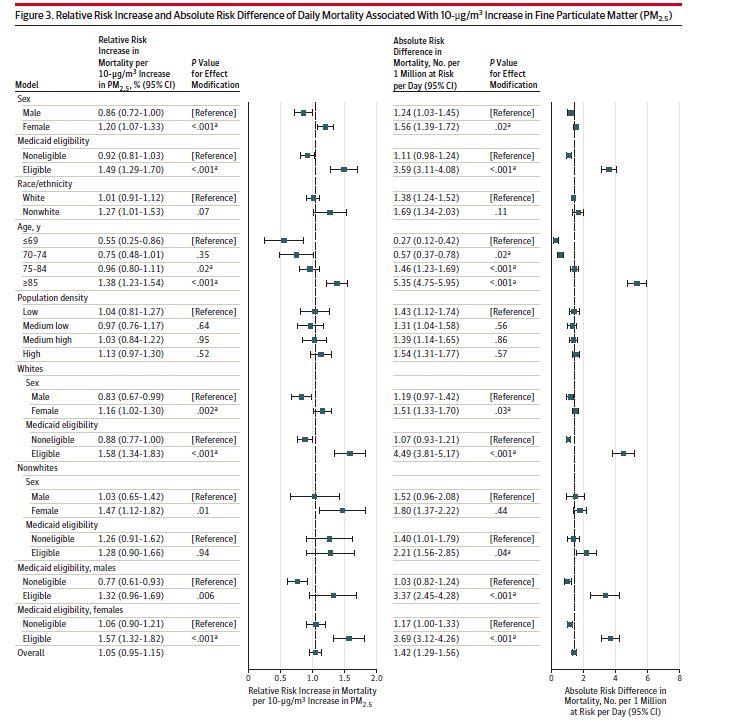
\includegraphics{p6.JPG}
\caption{Subgroup analysis of PM\(_{2.5}\)}
\end{figure}

\end{frame}

\begin{frame}{p-value}

two sample test
\(Z = \frac{RR_{male} - RR_{female}}{\sqrt{(se(RR_{male})^2 - se(RR_{female})^2)}}\)

\end{frame}

\begin{frame}{Dose-reponse}

\begin{figure}
\centering
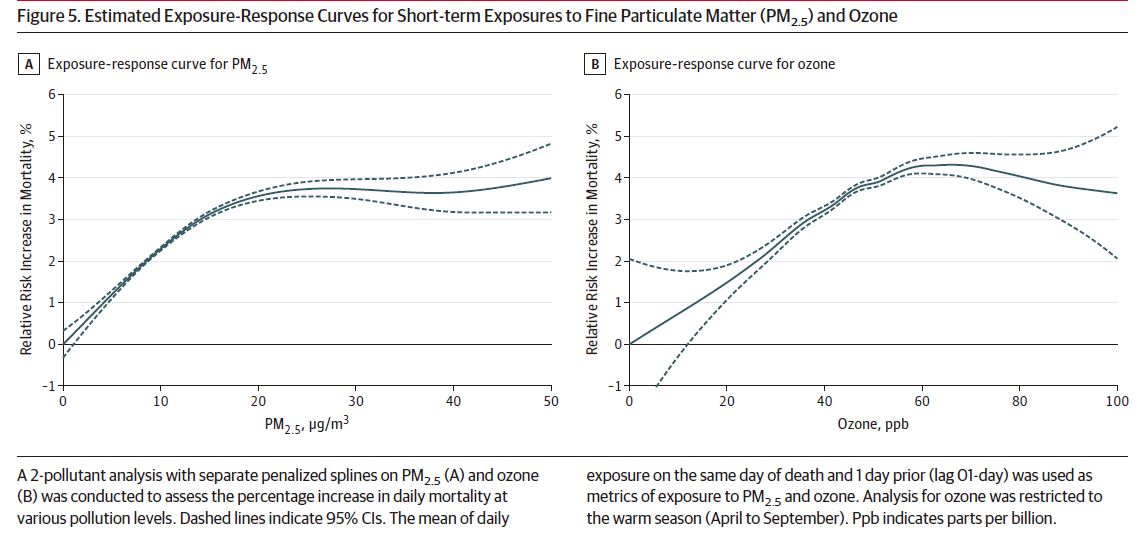
\includegraphics{p5.JPG}
\caption{Estimated Exposure-Response Curves for Short-term Exposures to
Fine Particulate Matter (PM\(_{2.5}\)) and Ozone}
\end{figure}

\end{frame}

\begin{frame}{Conclusions}

In the US Medicare population from 2000 to 2012, short-term exposures to
PM\(_{2.5}\) and warm-season ozone were significantly associated with
increased risk of mortality. This risk occurred at levels below current
national air quality standards, suggesting that these standards may need
to be reevaluated.

\end{frame}

\begin{frame}{}

Thanks!

\end{frame}

\end{document}
